\chapter{Nasadenie do vyučovania}
\label{chap:nasadenie_do_vyucovania}

Aby bola preverená celková kvalita virtuálneho laboratória, bol nástroj EVE-ng nasadený na vypracovávanie rôznych topológii z vybraných predmetov. 




\section{Používanie EVE-ng}
\label{chap:pouzivanie_eve_ng}

{\huge TODO - možno z tejto podkapitoly spraviť samostatnú kapitolu a dať ju pred nasadenie do vyučovania.}

Pre zvolené predmety boli vytvorené topológie podľa toho, aká téma bola na danom cvičení vyučovaná. Topológie boli vytvorené pomocou webového rozhrania EVE-ng, ktorým je možné spravovať topológie a používateľov. Predtým, než popíšeme výsledky pri nasadení na predmety, sa najprv budeme venovať vytváraniu topológii, ktoré nasadeniu predchádzali. Nižšie sú uvedené kroky na vytvorenie topológie v EVE-ng.

\begin{enumerate}[noitemsep]

    \item Najprv sa prihlásime do nástroja EVE-ng cez webové rozhranie v natívnom móde. Webové rozhranie je dostupné v 2 módoch: natívnom a HTML5. Rozdiely medzi jednotlivými módmi sú popísané v bode \ref{item:vzdialeny_pristup}. Pre úspešné prihlásenie musíme mať vytvorený používateľský účet, čo môže urobiť iba používateľ s rolou \emph{admin}.

{\huge TODO - obr. login screen s rozbaleným zoznamom módov}

    \item Po prihlásení sa zobrazí hlavná obrazovka. V ľavej časti je správca súborov, v ktorom si vyberieme adresár, kde sa súbor s topológiou bude nachádzať.

{\huge TODO - obr. main screen}

    \item Po výbere adresára klikneme na ikonku hárku s popisom \emph{Add new lab}, čím začneme vytváranie novej topológie. Topológiu môže vytvoriť iba používateľ s rolou \emph{editor} alebo \emph{admin}.

{\huge TODO - obr. main screen - lab toolbar}

    \item Zobrazí sa dialógové okno, do ktorého zadáme atribúty topológie.
    
{\huge TODO - popísať atribúty + ktoré sú povinné + obr. lab dialog}

    \item Po kliknutí na tlačidlo \emph{Save} sa súbor s topológiou vytvorí a následne sa zobrazí pracovná plocha na vytvorenie topológie. Zatiaľ je topológia prázdna.
    
{\huge TODO - obr. lab screen new}

    \item Do topológie môžeme pridávať tieto prvky:
    
    \begin{itemize}[noitemsep]
        \item Node - zariadenie
        \item Network - sieť
        \item Picture - obrázok
        \item Custom Shape - geometrický tvar - obdĺžnik/elipsa
        \item Text - textové polia
    \end{itemize}
    
    Spomenutý zoznam prvkov sa zobrazí v kontextovom menu po pravom kliknutí na prázdme miesto v topológii alebo po kliknutí na ikonku \emph{+}. {\huge TODO - obr. add a new object context menu}
    
    \item Po pridaní prvkov do topológie je s nimi možné ďalej pracovať. Každý z uvedených prvkov vieme upravovať rôznymi spôsobmi.
    
    \begin{itemize}[noitemsep]
        \item Najjednoduchším spôsobom úpravy platným pre všetky prvky je presunutie prvku myšou.
        \item Zariadenia je možné upravovať v zozname zariadení po kliknutí na položku \emph{Nodes} v menu na ľavej strane obrazovky. {\huge TODO - obr. Nodes dialog}.
        \item Ďalší spôsob, ako upraviť parametre zariadenia je pravým kliknutím na zariadenie a kliknutím na \emph{Edit}. {\huge TODO - obr. Edit dialog}.
        \item Siete sa dajú upravovať v zozname sietí po kliknutí na položku \emph{Networks} v menu na ľavej strane obrazovky. {\huge TODO - obr. Networks dialog}
        \item Obrázky, geometrické tvary a textové polia vieme upravovať v zozname objektov po kliknutí na položku \emph{Configured objects} v menu na ľavej strane obrazovky. {\huge TODO - obr. Configured objects dialog}
    \end{itemize}
    
Ďalší spôsob na úpravu prvkov v topológii je pomocou upravením samotného súboru s topológiou na serveri s príponou \emph{unl}. Tento súbor je napísaný vo formáte XML. Prvky sú definované značkami, ktoré definujú ich typ (zariadenie, textové pole a pod.). Nižšie je uvedený zoznam niektorých značiek a ich atribútov použitých v \emph{unl} súbore.

{\huge TODO - popísať značky}

    \begin{description}[noitemsep]
        \item \texttt{<node>}
        
        \begin{description}[noitemsep]
            \item \texttt{<interface>}
        \end{description}
        
        \item \texttt{<networks>}
        
        \begin{description}[noitemsep]
            \item \texttt{<network>}
        \end{description}
    \end{description}

Zmeny v \emph{unl} súbore sa prejavia až po znovunačítaní stránky (klávesou F5) alebo topológie (\emph{Refresh topology} v menu na ľavej strane obrazovky).

{\huge TODO - ukázať syntax UNL súboru zo servera na termináli}
    
    Experimentovaním sme zistili, že vytváranie topológii a duplikácia jej prvkov v \emph{unl} súbore je pomerne náročné, zdĺhavé a náchylné na chyby. Pri duplikácii zariadení bolo náročné udržať prehľad o.i. aj o identifikátoroch zariadení a rozhraní a ich vzájomnom prepojení v rámci. Výhodnejšie sa ukázalo najprv použiť webové rozhranie, potom tabuľku zariadení \emph{Nodes} a nakoniec upravovať \emph{unl} súbor:
    
    \begin{enumerate}[noitemsep]
        \item Najpr vo webovom rozhraní vytvoríme topológiu, pridáme do nej zariadenia a poprepájame ich.
        \item Potom v tabuľke zariadeníNodes (nazvy zariadeni)
        \item Ak je potrebné, nakoniec v \emph{unl} súbore presnejšie upravíme súradnice prvkov v topológii definovaných atribútmi \texttt{left} a \texttt{top}. Výsledkom týchto úprav je celkové zlepšenie estetickej úpravy. Môžeme tak urobiť aj vo webovom rozhraní v dialógovom okne pre úpravu zariadenia v atribútoch \emph{Left} a \emph{Top}, avšak v \emph{unl} súbore vieme súradnice prvkov upraviť hromadne.
    \end{enumerate}
    
    \item Potom, ako sme pridali zariadenia do topológie a poprepájali ich, môžeme zariadenia spustiť. Jednotlivé zariadenia môžeme spustiť:

{\huge TODO - po jednom}
{\huge TODO - vybraná skupina
      -Ctrl+klik -> pravy klik -> Start Selected
      -oznacenie mysou -> pravy klik -> Start selected}
{\huge TODO - Všetky zariadenia v topologii
      -More actions -> Start all nodes}
      
    \item \label{item:vzdialeny_pristup} Vzdialený prístup k zariadeniam 
    
        HTML5 mód zabezpečuje vzdialený prístup k zariadeniam pomocou reverzného proxy servera \emph{Apache Guacamole}, ktorý sa pripája na konzoly zariadení. HTML5 mód web rozhrania EVE-ng bol však menej stabilný a reagoval výrazne pomalšie pri práci s topológiou v provonaní s natívnym módom. Preto bolo webové rozhranie ďalej používané iba v natívnom móde.
        
        V HTML5 móde sa na obrazovke s otvorenou topológiou po kliknutí na zariadenie otvorí jeho vzdialená konzola. Avšak v natívnom móde potrebujeme mať pre otvorenie konzoly na zariadení nainštalované dodatočné nástroje na lokálnom počítači
        
{\huge TODO - popísať manuálny vzdialený prístup - telnet klient napr. putty a vnc klient napr. realvnc viewer}
        
{\huge TODO - popísať vzdialený prístup cez web interface - tzv. integračný balíček}
        
{\huge TODO - Popísať integračný balíček + rozdiely medzi predvoleným a upraveným integračným balíčkom}
        
{\huge TODO - Predvolená vs KIS verzia integračného balíčka -> SSH tunely (pre vzdialený prístup k zariadeniam v topológii)}

\end{enumerate}





\subsection{Prideľovanie portových čísel zariadeniam}
    automatické - vysvetliť, súbor node.php alebo tak nejako sa volá -> vzorec)
    ->rozsahy
    ->pridelovanie portovych cisel je sekvencne




\subsection{Pripojenie topológie k internetu / prepojenie topológii navzájom}

{\huge TODO - popísať pridávanie bridge network + podmienky konektivity (buď DHCP adresa alebo staticky nastavená a vo firewalle povolená) + obr. screenshot z topológie}






\section{Počítačové siete 2}

V rámci predmetu Počítačové siete 2 bol nástroj EVE-ng nasadený do vyučovania na vypracovávanie topológii s \emph{point-to-point} technológiami. Topológie boli spustené na fyzickom EVE-ng serveri. V prípade zlyhania EVE-ng boli pripravené aj záložné topológie v overenom nástroji Dynamips/Dynagen.

Najprv bola vytvorená základná topológia, znázornená na obrázku \ref{obr:eve_ng_ppp_zakladna_topo_v2}. Tá pozostávala zo štyroch Cisco IOL smerovačov a dvoch koncových zariadení s operačným systémom Alpine Linux. Cisco IOL smerovač bol vybraný, pretože ako jediný podporoval sériové rozhrania a \emph{point-to-point} technológie. Koncové zariadenie Alpine Linux bolo vybrané pre svoju nenáročnosť na systémové zdroje.

\begin{figure}
    \centering
    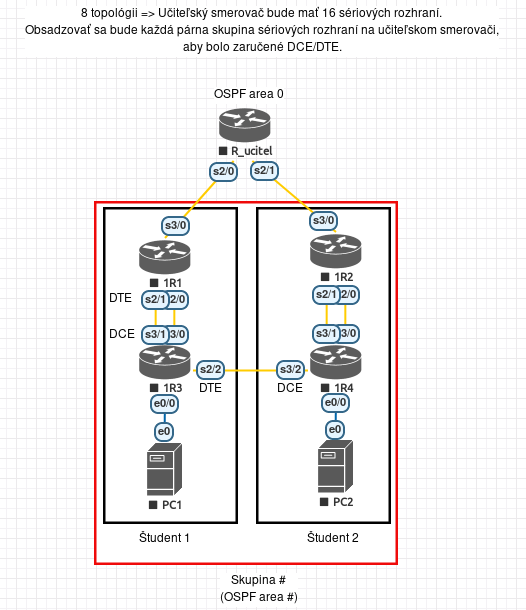
\includegraphics[width=0.75\textwidth]{eve_ng_ppp_zakladna_topo_v2}
    \caption{Základná PPP topológia}
    \label{obr:eve_ng_ppp_zakladna_topo_v2}
\end{figure}

Celkovo bolo vytvorených 8 zhodných topológii, ktoré medzi sebou zdieľali jeden učiteľský smerovač. V topológii sa celkovo nachádzalo 33 Cisco IOL smerovačov a 16 koncových staníc. Celková topológia sa nachádza na obrázku \ref{obr:eve_ng_ppp_celkova_topo_v2}.

\begin{figure}
    \centering
    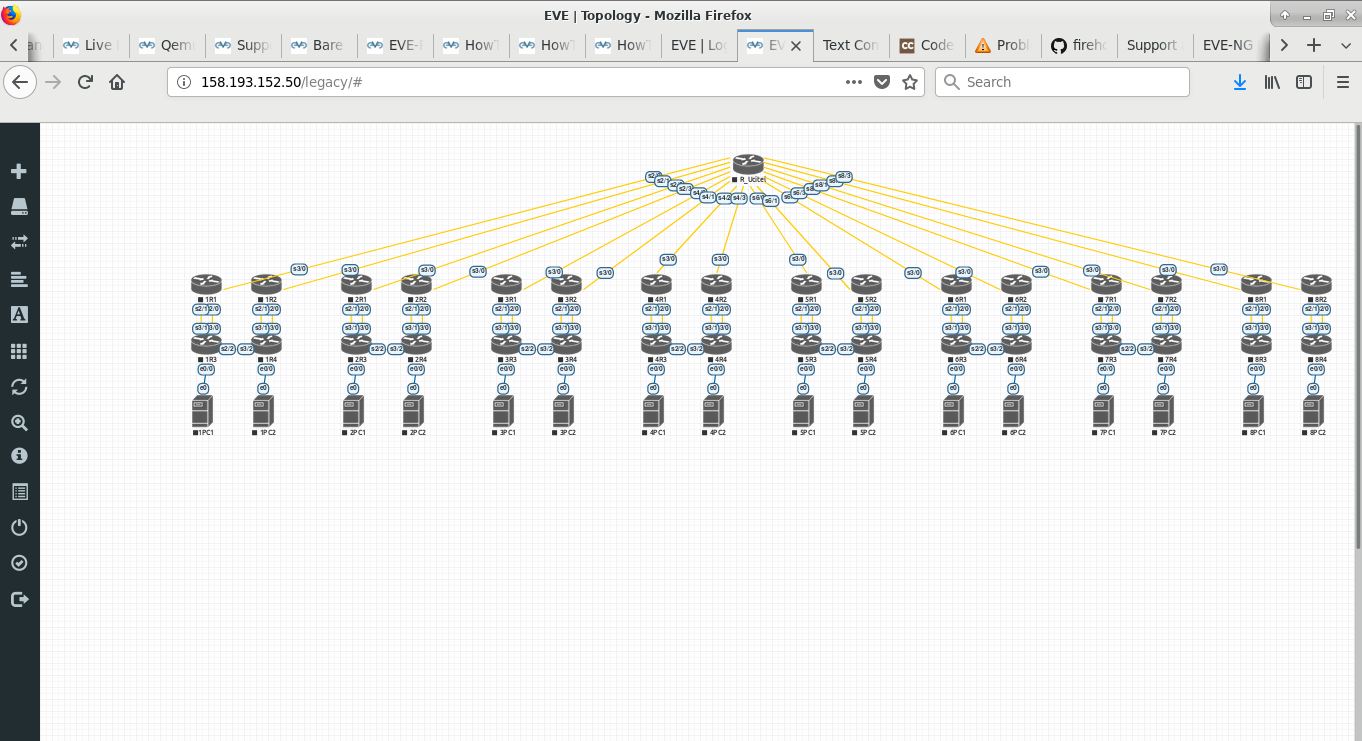
\includegraphics[width=0.75\textwidth]{eve_ng_ppp_celkova_topo_v2}
    \caption{Celková PPP topológia}
    \label{obr:eve_ng_ppp_celkova_topo_v2}
\end{figure}

IOL smerovače fungovali, až na príkaz \texttt{clock rate} na sériových rozhraniach, bez chyby. Ukázalo sa, že nastavenie DCE/DTE závisí od párnosti čísla skupiny. Párne číslo skupiny sériových rozhraní bude vždy DTE, nepárne vždy DCE, ako je zrejmé z obrázku \ref{obr:eve_ng_dce_dte_2E8S}. Rozdelenie sériových rozhraní na DCE/DTE nezávislé od počtu ethernetových alebo sériových skupín, čo potvrdzuje obrázok \ref{obr:eve_ng_dce_dte_1E8S}. Nastavenie DTE/DCE módu pre sériové rozhrania je v EVE-ng pri Cisco IOL smerovačoch pevne dané a nedá sa zmeniť, na čo treba myslieť pri návrhu topológie. V nástroji Dynamips/Dynagen sa dá DCE/DTE mód na jednotlivých sériových rozhraniach ľubovoľne meniť.

\begin{figure}
    \centering
    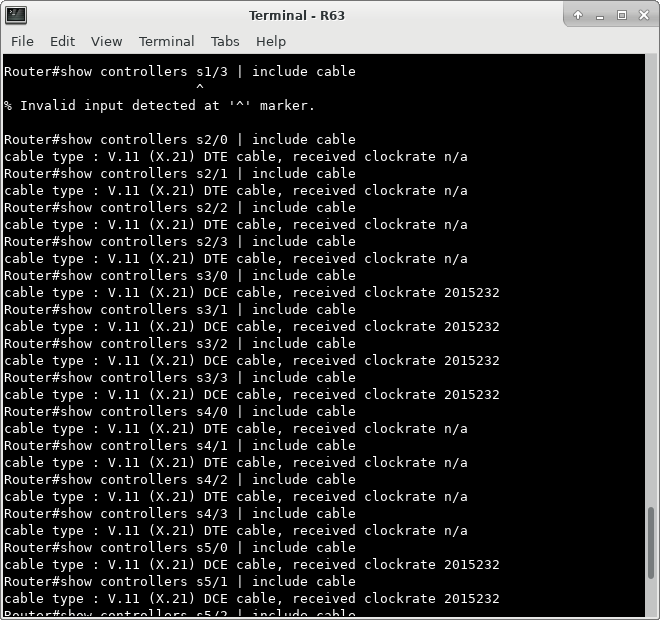
\includegraphics[width=0.75\textwidth]{eve_ng_dce_dte_2E8S}
    \caption{Typy sériových rozhraní na IOL smerovači - 2 ethernetové + 8 sériových skupín}
    \label{obr:eve_ng_dce_dte_2E8S}
\end{figure}

\begin{figure}
    \centering
    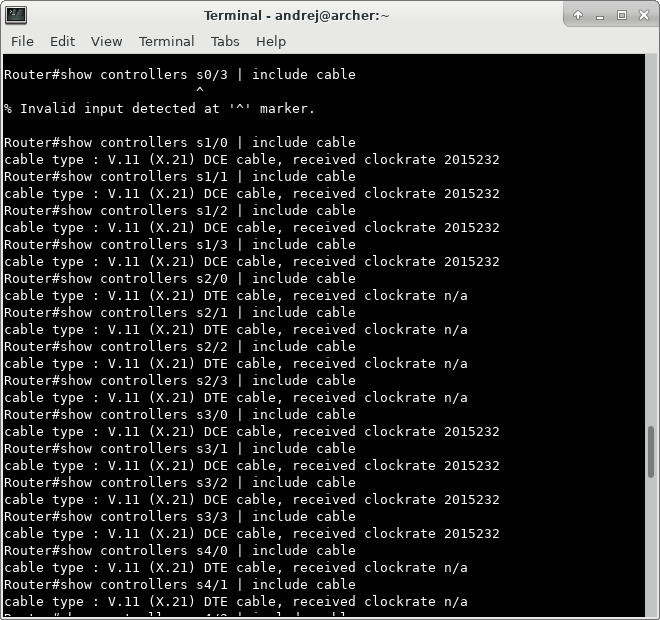
\includegraphics[width=0.75\textwidth]{eve_ng_dce_dte_1E8S}
    \caption{Typy sériových rozhraní na IOL smerovači - 1 ethernetová + 8 sériových skupín}
    \label{obr:eve_ng_dce_dte_1E8S}
\end{figure}

V jednej skupine sa vyskytol problém s jednosmernou PAP autentifikáciou študentského smerovača voči učiteľskému (R\_Ucitel(s4/1)-5R2(s2/1)). Príkaz \texttt{debug ppp authentication} hlásil chybu pri autentifikácii. Riešenie spočívalo v odstránení používateľa, vypnutí \emph{ppp} konfigurácie a vypnutí rozhraní. Tieto kroky boli vykonané aj na učiteľskom, aj na študentskom smerovači. Následne sa konektivita obnovila a spojenie pomocou PAP autentifikácie sa úspešne nadviazalo.

Je možné, že problémy vznikli aj kvôli tomu, že medzi študentským a učiteľským smerovačom boli na oboch stranách sériové rozhrania párnej skupiny t.j. obidva konce linky boli typu DTE. Niektoré skupiny študentov boli tiež pripojené k učiteľskému smerovaču sériovým rozhraním z párnej skupiny, ale takéto problémy nezaznamenali. Podobne tomu bolo aj pri prepojení Cisco IOL smerovačov rozhraniami DCE.

Z toho vyplýva, že Cisco IOL smerovače v EVE-ng majú pri prepojení dvoch smerovačov sériovou linkou s rovnakým módom nedefinované správanie. Tomu sa dá predísť vhodným návrhom topológie. Ten spočíva v tom, že sériové rozhrania medzi smerovačmi kombinujeme tak, aby bolo prepojené vždy sériové rozhranie párnej skupiny na jednom smerovači so sériovým rozhraním nepárnej skupiny na inom smerovači t.j. \emph{Serial2/x} (DCE) na prvom smerovači sa musí pripojiť napr. k \emph{Serial3/x} na druhom. V takom prípade DCE koniec po nastavení \texttt{clock rate} v príkaze \texttt{show controllers} zobrazí nastavený atribút \emph{received clockrate}, DTE koniec naproti tomu zobrazí hodnotu \emph{n/a}. Napriek tomu konektivita po správnom nastavení IP adries a zapnutí rozhranií bola aktívna.

Komplikácie s DCE/DTE a PPP autentifikáciou boli prítomné v prvom návrhu topológie, ktorý je znázornený na obrázku \ref{obr:eve_ng_ppp_zakladna_topo_v1}.

\begin{figure}
    \centering
    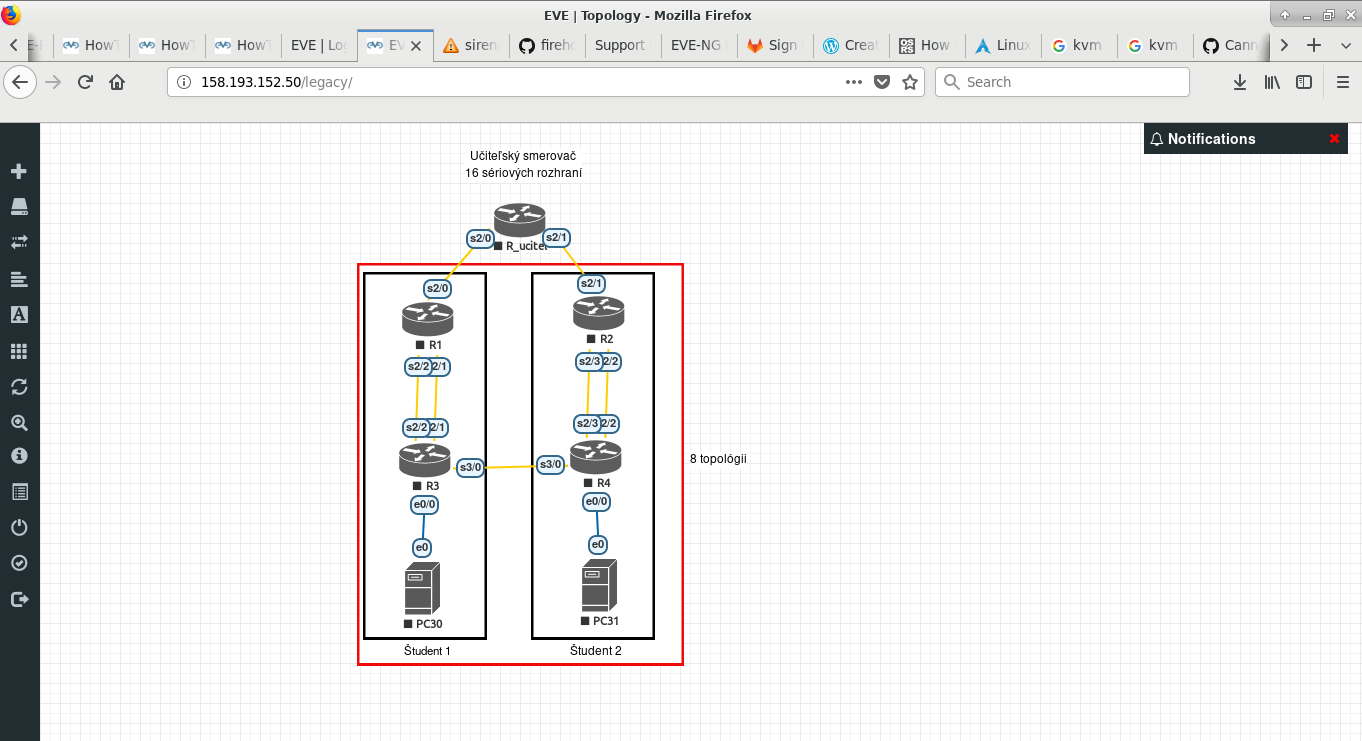
\includegraphics[width=0.75\textwidth]{eve_ng_ppp_zakladna_topo_v1}
    \caption{Základná PPP topológia - prvotný návrh}
    \label{obr:eve_ng_ppp_zakladna_topo_v1}
\end{figure}

Pri testovaní DCE/DTE rozhraní sme narazili na obmedzenie nástroja EVE-ng. Community verzia je totiž dovoľuje v jednej topológii mať spustených najviac 63 zariadení. Po spustení 64. sa na niekoľko sekúnd spustí, ale nakoniec sa automaticky vypne. Community verzia vie spustiť aj viac ako 64 zariadení v jednej topológii, ale vo výsledku sa spustia len niektoré, na prvý pohľad náhodne vybrané zariadenia. Avšak tie zariadenia, ktoré sa spustia, pracujú štandardným spôsobom. Uvedený problém sa nám nepodarilo vyriešiť ani rozšírením rozsahu portových čísel pre zariadenia v topológii.
  
Zmerané boli aj systémové požiadavky celkovej topológie na fyzickom EVE-ng serveri. Po vyhodnotení výsledkov merania sme zistili, že celá topológia, 33 Cisco IOL smerovačov a 16 koncových zariadení Alpine Linux, sa spúšťala približne 2 minúty, spotrebovala 13GB operačnej pamäte a procesor vyťažovala na 21\%. Celkovo by sme podľa celkového vyťaženia CPU mohli spustiť 4 takéto topológie, avšak množstvo operačnej pamäte dovoľovalo spustiť iba 3. Tabuľkový dokument s výsledkami merania je prítomný na CD v adresári \\ \emph{materialy\_na\_predmety/nasadenie\_do\_vyucovania/PS2/} v súbore \\ \emph{ps2\_7\_tyzden\_ppp\_topologia\_final\_8\_replik\_33\_IOL\_L3\_a\_16\_QEMU\_Alpine\_Linux.ods}.

Spomenutý súbor ukazuje veľké rozdiely v meraniach využitia operačnej pamäte medzi nástrojmi \emph{ps} a \emph{ps\_mem} v hárku \emph{VstupVystup}, hoci sa merala rovnaká množina procesov. Po manuálnom overení sa ukázalo, že prvý menovaný nástroj vykazoval presnejšie výsledky, preto boli pri odhadoch použité ním namerané hodnoty.





\section{Projektovanie sietí 1}

{\huge TODO -dorobiť budúci týždeň - konzultovať}

-nasadiť na jedno cvičenie Projektovania sietí 1
-1 používateľ môže mať otvorenú iba 1 topológiu, ktorá je obmedzená na 63 súčasne spustených zariadení. Ak treba mať spustených 100 smerovačov, 10 smerovačov v 10 topológiách, potom je potrebné vytvoriť 2 používateľské účty - polovicu topológii spustiť v jednom a polovicu v druhom používateľskom účte.





\section{Projektovanie sietí 2}

V rámci predmetu Počítačové siete 2 bol nástroj EVE-ng nasadený do vyučovania na vypracovávanie topológii s \emph{point-to-point} technológiami. Topológie boli spustené na virtuálnom VMware EVE-ng serveri.

V EVE-ng boli úspešne dokončené semestrálne práce s témou \emph{VPLS} a \emph{Seamless MPLS}. Téma \emph{EVPN} bola vypracovávaná v nástroji \emph{ViRo v2}.

Topológie semestrálnych prác sa skladali z týchto zariadení:

\begin{itemize}[noitemsep]
    \item Cisco IOL smerovač - VPLS, Seamless MPLS
    \item Cisco CSR - VPLS
    \item Juniper Olive - Seamless MPLS
    \item Juniper vMX 15 - VPLS
    \item Nokia VSR - EVPN
\end{itemize}





\section{Vyhodnotenie}

Z predmetov Počítačové siete 1, Pokročilé prepínanie v informačno-komunikačných sieťach a Pokročilé smerovanie v informačno-komunikačných sieťach neboli vypracované žiadne topológie.

Na predmetoch, kde nástroj EVE-ng nasadený bol, sa ukázalo, že ho je možné používať vo vyučovaní.

Študenti počas vypracovávaní topológie na predmete Počítačové siete 2 nezaznamenali žiadny rozdiel oproti nástroju Dynamips/Dynagen, keďže sa na zariadenia prihlasovali rovnako, pomocou nástroja \emph{PuTTY} IP adresou a portom, pričom zariadenia poskytovali rovnakú množinu funkcii, ako v nástroji Dynamips/Dynagen. Nástroj EVE-ng na fyzickom serveri bol počas celej doby vypracovávania stabilný.

Pri nasadení na predmet Projektovanie sietí 2, kde bola použitá virtuálna inštalácia EVE-ng, bol naopak nástroj nestabilný, zariadenia často zamŕzali a pri zadávaní príkazov do konzoly bola prítomná vyššia odozva z klávesnice. Mohlo to byť spôsobené mnohými faktormi, či už samotnou virtuálnou platformou VMware, alebo nesprávne nastavenými systémovými parametrami pre jednotlivé zariadenia v topológii.

Napriek mnohým nedostatkom nástroja EVE-ng, je výhodou vytvárať topológie z grafického rozhrania, namiesto z príkazového riadku. Nevýhodami sú nemožnosť stabilne spúšťať viac ako 63 zariadení v jednej topológii. Jednotliví používatelia a študenti si svoje topológie nemôžu spravovať nezávisle na sebe, keďže toto je možné iba v Learning Centre verzii nástroja.

Čo sa týka odhadov systémových požiadaviek topológii, tie môžeme odhadnúť súčtom systémových požiadaviek jednotlivých zariadení, ktoré sa v topológii budú nachádzať. Systémové požiadavky vybraných zariadení sú k dispozícii na CD v adresári \\ \emph{eve\_ng/profiling\_and\_benchmarking\_results/}.